\documentclass[journal,12pt,twocolumn]{IEEEtran}
%
\usepackage{setspace}
\usepackage{gensymb}
\singlespacing
\usepackage[cmex10]{amsmath}
\usepackage{amsthm}
\usepackage{mathrsfs}
\usepackage{txfonts}
\usepackage{stfloats}
\usepackage{bm}
\usepackage{cite}
\usepackage{cases}
\usepackage{subfig}
\usepackage{longtable}
\usepackage{multirow}
%\usepackage{algorithm}
\usepackage{enumitem}
\usepackage{mathtools}
\usepackage{steinmetz}
\usepackage{tikz}
\usepackage{circuitikz}
\usepackage{verbatim}
\usepackage{tfrupee}
\usepackage[breaklinks=true]{hyperref}
%\usepackage{stmaryrd}
\usepackage{tkz-euclide} % loads  TikZ and tkz-base
%\usetkzobj{all}
\usetikzlibrary{calc,math}
\usepackage{listings}
\usepackage{color}                                            %%
\usepackage{array}                                            %%
\usepackage{longtable}                                        %%
\usepackage{calc}                                             %%
\usepackage{multirow}                                         %%
\usepackage{hhline}                                           %%
\usepackage{ifthen}                                           %%
%optionally (for landscape tables embedded in another document): %%
\usepackage{lscape}     
\usepackage{multicol}
\usepackage{chngcntr}
%\usepackage{enumerate}

%\usepackage{wasysym}
%\newcounter{MYtempeqncnt}
\DeclareMathOperator*{\Res}{Res}
%\renewcommand{\baselinestretch}{2}
\renewcommand\thesection{\arabic{section}}
\renewcommand\thesubsection{\thesection.\arabic{subsection}}
\renewcommand\thesubsubsection{\thesubsection.\arabic{subsubsection}}
\newcommand\numberthis{\addtocounter{equation}{1}\tag{\theequation}}
\renewcommand\thesectiondis{\arabic{section}}
\renewcommand\thesubsectiondis{\thesectiondis.\arabic{subsection}}
\renewcommand\thesubsubsectiondis{\thesubsectiondis.\arabic{subsubsection}}

% correct bad hyphenation here
\hyphenation{op-tical net-works semi-conduc-tor}
\def\inputGnumericTable{}                                 %%

\lstset{
	%language=C,
	frame=single, 
	breaklines=true,
	columns=fullflexible
}


\begin{document}
	%
	
	
	\newtheorem{theorem}{Theorem}[section]
	\newtheorem{problem}{Problem}
	\newtheorem{proposition}{Proposition}[section]
	\newtheorem{lemma}{Lemma}[section]
	\newtheorem{corollary}[theorem]{Corollary}
	\newtheorem{example}{Example}[section]
	\newtheorem{definition}[problem]{Definition}
	
	\newcommand{\BEQA}{\begin{eqnarray}}
	\newcommand{\EEQA}{\end{eqnarray}}
	\newcommand{\define}{\stackrel{\triangle}{=}}
	\bibliographystyle{IEEEtran}
	%\bibliographystyle{ieeetr}
	\providecommand{\mbf}{\mathbf}
	\providecommand{\pr}[1]{\ensuremath{\Pr\left(#1\right)}}
	\providecommand{\qfunc}[1]{\ensuremath{Q\left(#1\right)}}
	\providecommand{\sbrak}[1]{\ensuremath{{}\left[#1\right]}}
	\providecommand{\lsbrak}[1]{\ensuremath{{}\left[#1\right.}}
	\providecommand{\rsbrak}[1]{\ensuremath{{}\left.#1\right]}}
	\providecommand{\brak}[1]{\ensuremath{\left(#1\right)}}
	\providecommand{\lbrak}[1]{\ensuremath{\left(#1\right.}}
	\providecommand{\rbrak}[1]{\ensuremath{\left.#1\right)}}
	\providecommand{\cbrak}[1]{\ensuremath{\left\{#1\right\}}}
	\providecommand{\lcbrak}[1]{\ensuremath{\left\{#1\right.}}
	\providecommand{\rcbrak}[1]{\ensuremath{\left.#1\right\}}}
	\theoremstyle{remark}
	\newtheorem{rem}{Remark}
	\newcommand{\sgn}{\mathop{\mathrm{sgn}}}
	\providecommand{\abs}[1]{\left\vert#1\right\vert}
	\providecommand{\res}[1]{\Res\displaylimits_{#1}} 
	\providecommand{\norm}[1]{\left\lVert#1\right\rVert}
	%\providecommand{\norm}[1]{\lVert#1\rVert}
	\providecommand{\mtx}[1]{\mathbf{#1}}
	\providecommand{\mean}[1]{E\left[ #1 \right]}
	\providecommand{\fourier}{\overset{\mathcal{F}}{ \rightleftharpoons}}
	%\providecommand{\hilbert}{\overset{\mathcal{H}}{ \rightleftharpoons}}
	\providecommand{\system}{\overset{\mathcal{H}}{ \longleftrightarrow}}
	%\newcommand{\solution}[2]{\textbf{Solution:}{#1}}
	\newcommand{\solution}{\noindent \textbf{Solution: }}
	\newcommand{\cosec}{\,\text{cosec}\,}
	\providecommand{\dec}[2]{\ensuremath{\overset{#1}{\underset{#2}{\gtrless}}}}
	\newcommand{\myvec}[1]{\ensuremath{\begin{pmatrix}#1\end{pmatrix}}}
	\newcommand{\mydet}[1]{\ensuremath{\begin{vmatrix}#1\end{vmatrix}}}
	\numberwithin{equation}{subsection}
	\makeatletter
	\@addtoreset{figure}{problem}
	\makeatother
	\let\StandardTheFigure\thefigure
	\let\vec\mathbf
	\renewcommand{\thefigure}{\theproblem}
	\def\putbox#1#2#3{\makebox[0in][l]{\makebox[#1][l]{}\raisebox{\baselineskip}[0in][0in]{\raisebox{#2}[0in][0in]{#3}}}}
	\def\rightbox#1{\makebox[0in][r]{#1}}
	\def\centbox#1{\makebox[0in]{#1}}
	\def\topbox#1{\raisebox{-\baselineskip}[0in][0in]{#1}}
	\def\midbox#1{\raisebox{-0.5\baselineskip}[0in][0in]{#1}}
	\vspace{3cm}
	\title{Matrix Theory Assignment 9}
	\author{Ritesh Kumar \\ EE20RESCH11005}
	
	
	\maketitle
	\newpage
	%\tableofcontents
	\bigskip
	\renewcommand{\thefigure}{\theenumi}
	\renewcommand{\thetable}{\theenumi}
	\counterwithout{figure}{section}
	\counterwithout{figure}{subsection}

	\date{Today}
	

\begin{abstract}
This problem demonstrate a method to  find nature linear transformation.
\end{abstract}
All the codes for the figure in this document can be found at
\begin{lstlisting}
https://github.com/Ritesh622/Assignment_EE5609/tree/master/Assignment_9
\end{lstlisting}
\section{\textbf{Problem}}
Let\textbf{T} and \textbf{U} be the linear operators  on $\mathbb{R}^2$  defined by 
\begin{align}
	\textbf{T}\brak{x_1,x_2} = \brak{x_2,x_1}\intertext{and} \textbf{U}\brak{x_1,x_2} = \brak{x_1,0 }
	\end{align}
	How would you describe T and U geometrically $?$

\section{solution}


Geometrically, in the x-y plane, \textbf{T} is the reflection about the diagonal x = y and \textbf{U} is a projection onto the x-axis.\\ 
\begin{align}
\intertext{Let Consider Matrix A as} \vec{A} = \myvec{0 & 1 \\ 1 & 0 } 
\end{align}
The matrix  $\vec{A}$ is representation  of the linear transformation T across the line y=x with respect to the standard basis.
\begin{align}
\intertext{Let suppose}\vec{x_1} = \myvec{1 \\ 2},\vec{x_2} = \myvec{3 \\ 4} 
\end{align}
After applying linear operator \textbf{T} on it,

\begin{align}
\textbf{T}\brak{x_1, x_2} = \vec{A}\myvec{\vec{x_1} & \vec{x_2}}\\
\implies   \vec{A}\myvec{\vec{x_1} & \vec{x_2}} =  \myvec{0 & 1 \\ 1 & 0 } \myvec{1 & 3 \\ 2 & 4} = \myvec{3 & 1 \\ 4 & 2}\\
%\end{align}
%\begin{align}
 \implies \vec{x_1} = \myvec{3 \\ 4}, \vec{x_2} = \myvec{1 \\ 2}
\end{align}

\begin{figure}[htb!]	
	\centering	
	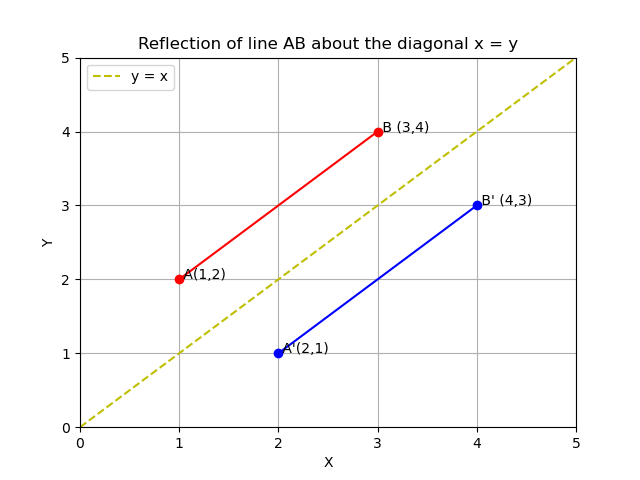
\includegraphics[width=\columnwidth]{Reflection.png}	
	\caption{Reflection of line AB about the  x = y}
	\label{fig1}	
\end{figure}
\begin{figure}[htb!]	
	\centering	
	\includegraphics[width=\columnwidth]{Projection1.png}	
	\caption{Projection of AB onto x-axis}
	\label{fig2}	
\end{figure}

After applying linear operator \textbf{U} on it,
\begin{align}
\vec{x_1} = \myvec{1 \\ 2}, \vec{x_2} = \myvec{0 \\ 0}
\end{align}


\begin{align}
\textbf{T}\brak{x_1, x_2} = \vec{A}\myvec{\vec{x_1} & \vec{x_2}}\\
\implies   \vec{A}\myvec{\vec{x_1} & \vec{x_2}} =  \myvec{1 &  0\\ 0 & 0 } \myvec{1 & 3 \\ 2 & 4} = \myvec{1 & 3 \\ 0 & 0}\\
%\end{align}
%\begin{align}
\implies \vec{x_1} = \myvec{1 \\ 0}, \vec{x_2} = \myvec{3 \\ 0}
\end{align}


\end{document}